% Function to generate color based on percentage value
\newcommand{\cellcolorpercent}[1]{%
  \ifdim #1 pt < 10 pt \cellcolor{red!90}%
  \else\ifdim #1 pt < 20 pt \cellcolor{red!80}%
  \else\ifdim #1 pt < 30 pt \cellcolor{red!70}%
  \else\ifdim #1 pt < 40 pt \cellcolor{red!60}%
  \else\ifdim #1 pt < 50 pt \cellcolor{red!50}%
  \else\ifdim #1 pt < 60 pt \cellcolor{yellow!40}%
  \else\ifdim #1 pt < 70 pt \cellcolor{yellow!30}%
  \else\ifdim #1 pt < 80 pt \cellcolor{green!30}%
  \else\ifdim #1 pt < 90 pt \cellcolor{green!50}%
  \else\ifdim #1 pt < 100 pt \cellcolor{green!70}%
  \else\cellcolor{green!90}%
  \fi\fi\fi\fi\fi\fi\fi\fi\fi\fi
}

\makeatletter
\newcommand{\thickhline}{%
    \noalign {\ifnum 0=`}\fi \hrule height 3pt
    \futurelet \reserved@a \@xhline
}
\newcolumntype{"}{@{\hskip\tabcolsep\vrule width 1pt\hskip\tabcolsep}}
\makeatother

\renewcommand{\arraystretch}{1.5}
\begin{table}[ht]
\centering
\begin{tabular}{|>{\arraybackslash}p{5cm}|>{\arraybackslash}p{1.5cm}|c|c|c|c|}
\hline
\rowcolor[HTML]{C0C0C0}
\textbf{} & \textbf{Iteration} & \textbf{0} & \textbf{1} & \textbf{2} & \textbf{3} \\ \hline
Win Condition Recognition & 
\includegraphics[scale=0.07]{figs/emojis/emoji_1.png} & \cellcolorpercent{35.0} \textbf{35.0\%} & \cellcolorpercent{55.0} \textbf{55.0\%} & \cellcolorpercent{87.5} \textbf{87.5\%} & \cellcolorpercent{87.5} \textbf{87.5\%} \\ \hline
Rule Modification & 
\includegraphics[scale=0.07]{figs/emojis/emoji_2.png} & \cellcolorpercent{0.0} \textbf{0.0\%} & \cellcolorpercent{10.0} \textbf{10.0\%} & \cellcolorpercent{37.5} \textbf{37.5\%} & \cellcolorpercent{61.9} \textbf{61.9\%} \\ \hline
Direct Navigation Efficiency & 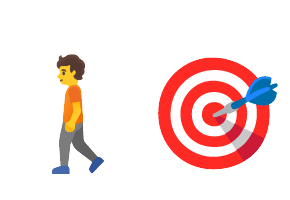
\includegraphics[scale=0.07]{figs/emojis/emoji_3.png} & \cellcolorpercent{5.6} \textbf{5.6\%} & \cellcolorpercent{22.5} \textbf{22.5\%} & \cellcolorpercent{27.5} \textbf{27.5\%} & \cellcolorpercent{37.5} \textbf{37.5\%} \\ \hline
Context-Sensitive Decision Making & 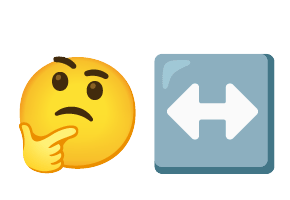
\includegraphics[scale=0.07]{figs/emojis/emoji_4.png} & \cellcolorpercent{2.5} \textbf{2.5\%} & \cellcolorpercent{27.5} \textbf{27.5\%} & \cellcolorpercent{30.0} \textbf{30.0\%} & \cellcolorpercent{37.5} \textbf{37.5\%} \\ \hline
Win Rule Construction & 
\includegraphics[scale=0.07]{figs/emojis/emoji_5.png} & \cellcolor[gray]{0.85} 0.0\% & \cellcolorpercent{0.0} \textbf{0.0\%} & \cellcolorpercent{0.0} \textbf{0.0\%} & \cellcolorpercent{5.3} \textbf{5.3\%} \\ \hline
Selective Interaction With Relevant Objects & 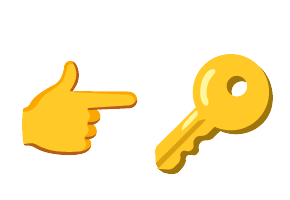
\includegraphics[scale=0.07]{figs/emojis/emoji_6.png} & \cellcolor[gray]{0.85} 35.0\% & \cellcolorpercent{40.0} \textbf{40.0\%} & \cellcolorpercent{45.0} \textbf{45.0\%} & \cellcolorpercent{82.5} \textbf{82.5\%} \\ \hline
Rule Manipulation and Execution & 
\includegraphics[scale=0.07]{figs/emojis/emoji_7.png} & \cellcolor[gray]{0.85} 0.0\% & \cellcolorpercent{12.5} \textbf{12.5\%} & \cellcolorpercent{31.0} \textbf{31.0\%} & \cellcolorpercent{35.5} \textbf{35.5\%} \\ \hline
Subtask Coordination & 
\includegraphics[scale=0.07]{figs/emojis/emoji_8.png} & \cellcolor[gray]{0.85} 2.5\% & \cellcolor[gray]{0.85} 25.0\% & \cellcolorpercent{27.5} \textbf{27.5\%} & \cellcolorpercent{35.0} \textbf{35.0\%} \\ \hline
Immovable Interaction & 
\includegraphics[scale=0.07]{figs/emojis/emoji_9.png} & \cellcolor[gray]{0.85} 64.9\% & \cellcolor[gray]{0.85} 69.7\% & \cellcolor[gray]{0.85} 69.7\% & \cellcolorpercent{87.9} \textbf{87.9\%} \\
\thickhline
\multicolumn{2}{|c|}{Coverage} & \textbf{65.0\%} & \textbf{83.0\%} & \textbf{85.0\%} & \textbf{92.0\%} \\ \hline
\multicolumn{2}{|c|}{Redundancy} & \textbf{58.0\%} & \textbf{59.0\%} & \textbf{47.0\%} & \textbf{59.0\%} \\ \hline
\end{tabular}
\caption{Metric Performance for baba-is-ai AutoLibra Iterations 0–3, Across Full (40) Environment Tasks}
\label{tab:metric_perf}
\end{table}
    